% ------------------------------------------------------------------------
%  sparse_matrix_template memory fix: std::map -> boost::container::flat_map.
%  Hand-authored from the 2026-09-01 matched pair (rank 1, 6VYB, 4 MPI ranks,
%  LIS -- verified in both captures, not taken from the filenames):
%  test1/profiles/ngpb.rank1.zst (std::map, captured 17:38 against a
%  reinstalled base bimpp) and the cook of the 13:43 capture (flat_map).
%  Same config, VERIFIED -- not assumed. The container-independent mesh proxies
%  are identical digit for digit across the pair:
%      num_local_nodes  813.29M over 726488 calls   (both)
%      create_density_map    84882360 calls         (both)
%  and the whole 7.69M difference in total allocation count is accounted for by
%  the 7.71M difference at the assembly container site, to within 20k of 599M.
%  The superseded pair (base.zst / opt.amgx.zst, Apr+May) was NOT same-config:
%  those proxies differed by 13.5%, which inflated the drop. Do not go back.
%
%  TOTALS are heaptrack_print / Summary "peak heap memory consumption", NOT the
%  Top-Down "main" row. Top-Down main is not the process peak -- the tree has
%  several roots (main, _start, __clone3) and merged-node peaks are documented
%  as "not correct"; captures can also unwind to different depths and root the
%  same allocation differently, which silently drops it from main's subtree.
%  ASSEMBLY bars sum the peak consumers heaptrack_print reports under
%  --filter-bt-function assemble_system_matrix. Two sites dominate:
%      entry storage      2.40G -> 1.02G   (RB-tree nodes -> flat vectors)
%      row-handle array   1.34G -> 672.21M (one alloc; 48B -> 24B per row)
%  everything else is under 60MB. This inherits the merged-peak caveat (maxima
%  at different instants), unlike the totals, which are exact.
%  See [[project_bimpp_memory]].
%  Include with % ------------------------------------------------------------------------
%  sparse_matrix_template memory fix: std::map -> boost::container::flat_map.
%  Hand-authored from the 2026-09-01 matched pair (rank 1, 6VYB, 4 MPI ranks,
%  LIS -- verified in both captures, not taken from the filenames):
%  test1/profiles/ngpb.rank1.zst (std::map, captured 17:38 against a
%  reinstalled base bimpp) and the cook of the 13:43 capture (flat_map).
%  Same config, VERIFIED -- not assumed. The container-independent mesh proxies
%  are identical digit for digit across the pair:
%      num_local_nodes  813.29M over 726488 calls   (both)
%      create_density_map    84882360 calls         (both)
%  and the whole 7.69M difference in total allocation count is accounted for by
%  the 7.71M difference at the assembly container site, to within 20k of 599M.
%  The superseded pair (base.zst / opt.amgx.zst, Apr+May) was NOT same-config:
%  those proxies differed by 13.5%, which inflated the drop. Do not go back.
%
%  TOTALS are heaptrack_print / Summary "peak heap memory consumption", NOT the
%  Top-Down "main" row. Top-Down main is not the process peak -- the tree has
%  several roots (main, _start, __clone3) and merged-node peaks are documented
%  as "not correct"; captures can also unwind to different depths and root the
%  same allocation differently, which silently drops it from main's subtree.
%  ASSEMBLY bars sum the peak consumers heaptrack_print reports under
%  --filter-bt-function assemble_system_matrix. Two sites dominate:
%      entry storage      2.40G -> 1.02G   (RB-tree nodes -> flat vectors)
%      row-handle array   1.34G -> 672.21M (one alloc; 48B -> 24B per row)
%  everything else is under 60MB. This inherits the merged-peak caveat (maxima
%  at different instants), unlike the totals, which are exact.
%  See [[project_bimpp_memory]].
%  Include with % ------------------------------------------------------------------------
%  sparse_matrix_template memory fix: std::map -> boost::container::flat_map.
%  Hand-authored from the 2026-09-01 matched pair (rank 1, 6VYB, 4 MPI ranks,
%  LIS -- verified in both captures, not taken from the filenames):
%  test1/profiles/ngpb.rank1.zst (std::map, captured 17:38 against a
%  reinstalled base bimpp) and the cook of the 13:43 capture (flat_map).
%  Same config, VERIFIED -- not assumed. The container-independent mesh proxies
%  are identical digit for digit across the pair:
%      num_local_nodes  813.29M over 726488 calls   (both)
%      create_density_map    84882360 calls         (both)
%  and the whole 7.69M difference in total allocation count is accounted for by
%  the 7.71M difference at the assembly container site, to within 20k of 599M.
%  The superseded pair (base.zst / opt.amgx.zst, Apr+May) was NOT same-config:
%  those proxies differed by 13.5%, which inflated the drop. Do not go back.
%
%  TOTALS are heaptrack_print / Summary "peak heap memory consumption", NOT the
%  Top-Down "main" row. Top-Down main is not the process peak -- the tree has
%  several roots (main, _start, __clone3) and merged-node peaks are documented
%  as "not correct"; captures can also unwind to different depths and root the
%  same allocation differently, which silently drops it from main's subtree.
%  ASSEMBLY bars sum the peak consumers heaptrack_print reports under
%  --filter-bt-function assemble_system_matrix. Two sites dominate:
%      entry storage      2.40G -> 1.02G   (RB-tree nodes -> flat vectors)
%      row-handle array   1.34G -> 672.21M (one alloc; 48B -> 24B per row)
%  everything else is under 60MB. This inherits the merged-peak caveat (maxima
%  at different instants), unlike the totals, which are exact.
%  See [[project_bimpp_memory]].
%  Include with % ------------------------------------------------------------------------
%  sparse_matrix_template memory fix: std::map -> boost::container::flat_map.
%  Hand-authored from the 2026-09-01 matched pair (rank 1, 6VYB, 4 MPI ranks,
%  LIS -- verified in both captures, not taken from the filenames):
%  test1/profiles/ngpb.rank1.zst (std::map, captured 17:38 against a
%  reinstalled base bimpp) and the cook of the 13:43 capture (flat_map).
%  Same config, VERIFIED -- not assumed. The container-independent mesh proxies
%  are identical digit for digit across the pair:
%      num_local_nodes  813.29M over 726488 calls   (both)
%      create_density_map    84882360 calls         (both)
%  and the whole 7.69M difference in total allocation count is accounted for by
%  the 7.71M difference at the assembly container site, to within 20k of 599M.
%  The superseded pair (base.zst / opt.amgx.zst, Apr+May) was NOT same-config:
%  those proxies differed by 13.5%, which inflated the drop. Do not go back.
%
%  TOTALS are heaptrack_print / Summary "peak heap memory consumption", NOT the
%  Top-Down "main" row. Top-Down main is not the process peak -- the tree has
%  several roots (main, _start, __clone3) and merged-node peaks are documented
%  as "not correct"; captures can also unwind to different depths and root the
%  same allocation differently, which silently drops it from main's subtree.
%  ASSEMBLY bars sum the peak consumers heaptrack_print reports under
%  --filter-bt-function assemble_system_matrix. Two sites dominate:
%      entry storage      2.40G -> 1.02G   (RB-tree nodes -> flat vectors)
%      row-handle array   1.34G -> 672.21M (one alloc; 48B -> 24B per row)
%  everything else is under 60MB. This inherits the merged-peak caveat (maxima
%  at different instants), unlike the totals, which are exact.
%  See [[project_bimpp_memory]].
%  Include with \input{figures/bimpp_memory_fix}
%  Needs \usepackage{pgfplots} in the preamble.
% ------------------------------------------------------------------------
\pgfplotsset{compat=1.16}

\definecolor{memtotal}{HTML}{2C5F8D}
\definecolor{memassemble}{HTML}{9DC3E0}

\begin{figure}[!htb]
\centering
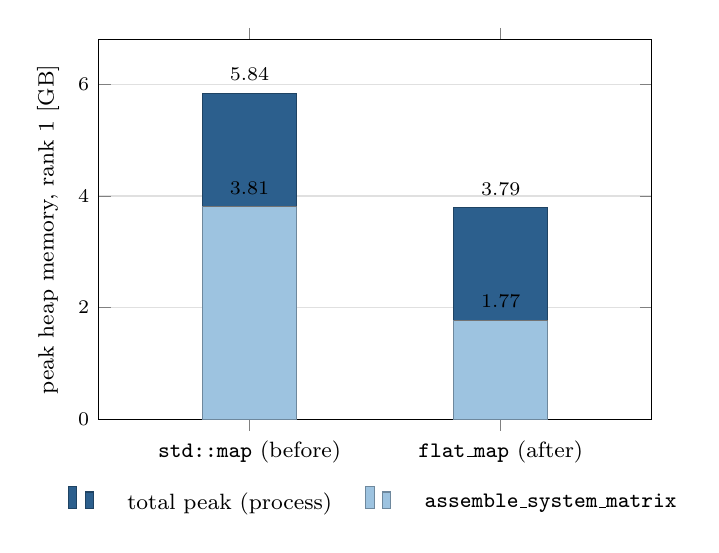
\begin{tikzpicture}
\begin{axis}[
    ybar,
    width=8.6cm, height=6.4cm,
    bar width=34pt,
    xmin=-0.6, xmax=1.6,
    xtick={0,1},
    xticklabels={\texttt{std::map} (before),\texttt{flat\_map} (after)},
    xticklabel style={font=\footnotesize, align=center},
    ymin=0, ymax=6.8,
    ylabel={peak heap memory, rank 1 [GB]},
    ylabel style={font=\footnotesize},
    tick label style={font=\scriptsize},
    ymajorgrids=true,
    major grid style={black!12},
    legend style={
      at={(0.5,-0.16)}, anchor=north, draw=none,
      legend columns=2, font=\footnotesize, column sep=1em,
    },
]
  % Overlay, not stack: assemble_system_matrix is a subset of the total, so the
  % second series is drawn at the same x position (bar shift=0pt) on top of the
  % first, covering its lower portion. The remaining visible strip of memtotal
  % above the seam is "everything in main's peak that is not assembly".
  \addplot+[
    ybar, bar shift=0pt, fill=memtotal, draw=memtotal!70!black, line width=0.4pt,
  ] coordinates {(0,5.84) (1,3.79)};
  \addlegendentry{total peak (process)}
  \addplot+[
    ybar, bar shift=0pt, fill=memassemble, draw=memassemble!70!black, line width=0.4pt,
  ] coordinates {(0,3.81) (1,1.77)};
  \addlegendentry{\texttt{assemble\_system\_matrix}}

  % Value labels: total at the bar top, assemble at the seam between the two
  % colors, with a short cap line marking the seam itself.
  \node[font=\scriptsize, anchor=south, yshift=1pt] at (axis cs:0,5.84) {5.84};
  \node[font=\scriptsize, anchor=south, yshift=1pt] at (axis cs:1,3.79) {3.79};
  \draw[black!55, line width=0.6pt] ([xshift=-17pt]axis cs:0,3.81) -- ([xshift=17pt]axis cs:0,3.81);
  \draw[black!55, line width=0.6pt] ([xshift=-17pt]axis cs:1,1.77) -- ([xshift=17pt]axis cs:1,1.77);
  \node[font=\scriptsize, anchor=south, yshift=1pt] at (axis cs:0,3.81) {3.81};
  \node[font=\scriptsize, anchor=south, yshift=1pt] at (axis cs:1,1.77) {1.77};
\end{axis}
\end{tikzpicture}

\caption[Sparse matrix memory fix]{\textbf{Effect of the \texttt{sparse\_matrix\_template} fix on peak host memory, 6VYB, rank 1.} The process-wide peak heap consumption against the peak attributable to \snakecase{assemble\_system\_matrix} (Section~\ref{sec:evaluation-experimental-setup-comparing-memory-utilization}). Both captures use the LIS solver, measured on the local system (Table~\ref{tab:test-systems}).}
\label{fig:bimpp-memory-fix}
\end{figure}

%  Needs \usepackage{pgfplots} in the preamble.
% ------------------------------------------------------------------------
\pgfplotsset{compat=1.16}

\definecolor{memtotal}{HTML}{2C5F8D}
\definecolor{memassemble}{HTML}{9DC3E0}

\begin{figure}[!htb]
\centering
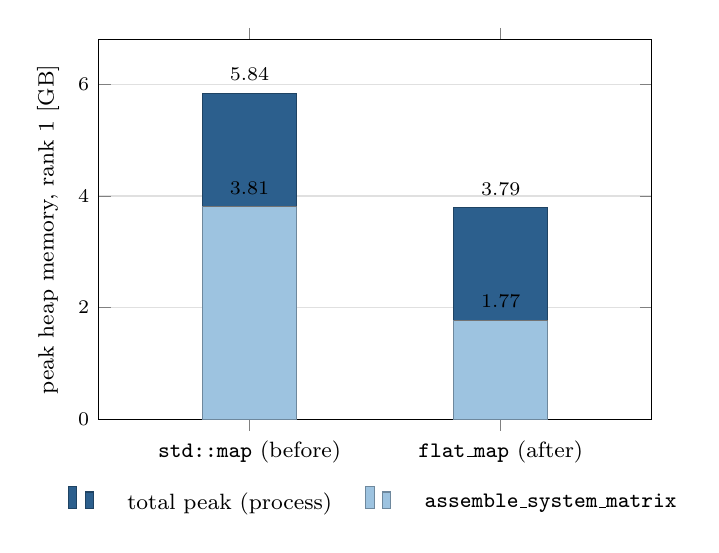
\begin{tikzpicture}
\begin{axis}[
    ybar,
    width=8.6cm, height=6.4cm,
    bar width=34pt,
    xmin=-0.6, xmax=1.6,
    xtick={0,1},
    xticklabels={\texttt{std::map} (before),\texttt{flat\_map} (after)},
    xticklabel style={font=\footnotesize, align=center},
    ymin=0, ymax=6.8,
    ylabel={peak heap memory, rank 1 [GB]},
    ylabel style={font=\footnotesize},
    tick label style={font=\scriptsize},
    ymajorgrids=true,
    major grid style={black!12},
    legend style={
      at={(0.5,-0.16)}, anchor=north, draw=none,
      legend columns=2, font=\footnotesize, column sep=1em,
    },
]
  % Overlay, not stack: assemble_system_matrix is a subset of the total, so the
  % second series is drawn at the same x position (bar shift=0pt) on top of the
  % first, covering its lower portion. The remaining visible strip of memtotal
  % above the seam is "everything in main's peak that is not assembly".
  \addplot+[
    ybar, bar shift=0pt, fill=memtotal, draw=memtotal!70!black, line width=0.4pt,
  ] coordinates {(0,5.84) (1,3.79)};
  \addlegendentry{total peak (process)}
  \addplot+[
    ybar, bar shift=0pt, fill=memassemble, draw=memassemble!70!black, line width=0.4pt,
  ] coordinates {(0,3.81) (1,1.77)};
  \addlegendentry{\texttt{assemble\_system\_matrix}}

  % Value labels: total at the bar top, assemble at the seam between the two
  % colors, with a short cap line marking the seam itself.
  \node[font=\scriptsize, anchor=south, yshift=1pt] at (axis cs:0,5.84) {5.84};
  \node[font=\scriptsize, anchor=south, yshift=1pt] at (axis cs:1,3.79) {3.79};
  \draw[black!55, line width=0.6pt] ([xshift=-17pt]axis cs:0,3.81) -- ([xshift=17pt]axis cs:0,3.81);
  \draw[black!55, line width=0.6pt] ([xshift=-17pt]axis cs:1,1.77) -- ([xshift=17pt]axis cs:1,1.77);
  \node[font=\scriptsize, anchor=south, yshift=1pt] at (axis cs:0,3.81) {3.81};
  \node[font=\scriptsize, anchor=south, yshift=1pt] at (axis cs:1,1.77) {1.77};
\end{axis}
\end{tikzpicture}

\caption[Sparse matrix memory fix]{\textbf{Effect of the \texttt{sparse\_matrix\_template} fix on peak host memory, 6VYB, rank 1.} The process-wide peak heap consumption against the peak attributable to \snakecase{assemble\_system\_matrix} (Section~\ref{sec:evaluation-experimental-setup-comparing-memory-utilization}). Both captures use the LIS solver, measured on the local system (Table~\ref{tab:test-systems}).}
\label{fig:bimpp-memory-fix}
\end{figure}

%  Needs \usepackage{pgfplots} in the preamble.
% ------------------------------------------------------------------------
\pgfplotsset{compat=1.16}

\definecolor{memtotal}{HTML}{2C5F8D}
\definecolor{memassemble}{HTML}{9DC3E0}

\begin{figure}[!htb]
\centering
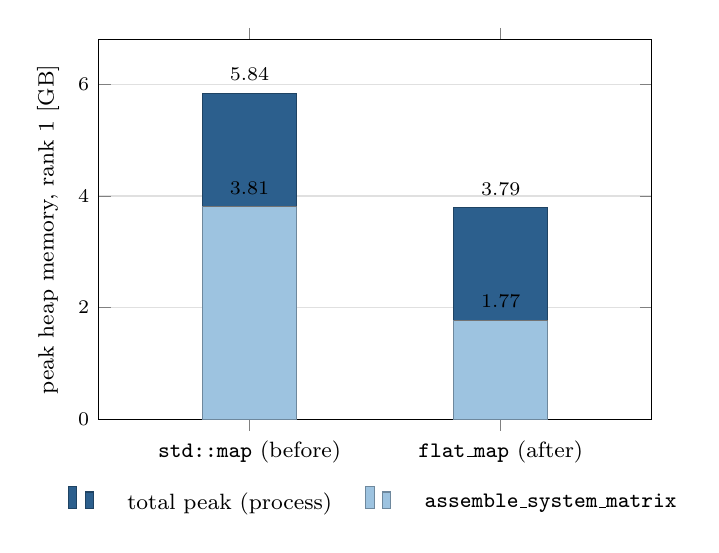
\begin{tikzpicture}
\begin{axis}[
    ybar,
    width=8.6cm, height=6.4cm,
    bar width=34pt,
    xmin=-0.6, xmax=1.6,
    xtick={0,1},
    xticklabels={\texttt{std::map} (before),\texttt{flat\_map} (after)},
    xticklabel style={font=\footnotesize, align=center},
    ymin=0, ymax=6.8,
    ylabel={peak heap memory, rank 1 [GB]},
    ylabel style={font=\footnotesize},
    tick label style={font=\scriptsize},
    ymajorgrids=true,
    major grid style={black!12},
    legend style={
      at={(0.5,-0.16)}, anchor=north, draw=none,
      legend columns=2, font=\footnotesize, column sep=1em,
    },
]
  % Overlay, not stack: assemble_system_matrix is a subset of the total, so the
  % second series is drawn at the same x position (bar shift=0pt) on top of the
  % first, covering its lower portion. The remaining visible strip of memtotal
  % above the seam is "everything in main's peak that is not assembly".
  \addplot+[
    ybar, bar shift=0pt, fill=memtotal, draw=memtotal!70!black, line width=0.4pt,
  ] coordinates {(0,5.84) (1,3.79)};
  \addlegendentry{total peak (process)}
  \addplot+[
    ybar, bar shift=0pt, fill=memassemble, draw=memassemble!70!black, line width=0.4pt,
  ] coordinates {(0,3.81) (1,1.77)};
  \addlegendentry{\texttt{assemble\_system\_matrix}}

  % Value labels: total at the bar top, assemble at the seam between the two
  % colors, with a short cap line marking the seam itself.
  \node[font=\scriptsize, anchor=south, yshift=1pt] at (axis cs:0,5.84) {5.84};
  \node[font=\scriptsize, anchor=south, yshift=1pt] at (axis cs:1,3.79) {3.79};
  \draw[black!55, line width=0.6pt] ([xshift=-17pt]axis cs:0,3.81) -- ([xshift=17pt]axis cs:0,3.81);
  \draw[black!55, line width=0.6pt] ([xshift=-17pt]axis cs:1,1.77) -- ([xshift=17pt]axis cs:1,1.77);
  \node[font=\scriptsize, anchor=south, yshift=1pt] at (axis cs:0,3.81) {3.81};
  \node[font=\scriptsize, anchor=south, yshift=1pt] at (axis cs:1,1.77) {1.77};
\end{axis}
\end{tikzpicture}

\caption[Sparse matrix memory fix]{\textbf{Effect of the \texttt{sparse\_matrix\_template} fix on peak host memory, 6VYB, rank 1.} The process-wide peak heap consumption against the peak attributable to \snakecase{assemble\_system\_matrix} (Section~\ref{sec:evaluation-experimental-setup-comparing-memory-utilization}). Both captures use the LIS solver, measured on the local system (Table~\ref{tab:test-systems}).}
\label{fig:bimpp-memory-fix}
\end{figure}

%  Needs \usepackage{pgfplots} in the preamble.
% ------------------------------------------------------------------------
\pgfplotsset{compat=1.16}

\definecolor{memtotal}{HTML}{2C5F8D}
\definecolor{memassemble}{HTML}{9DC3E0}

\begin{figure}[!htb]
\centering
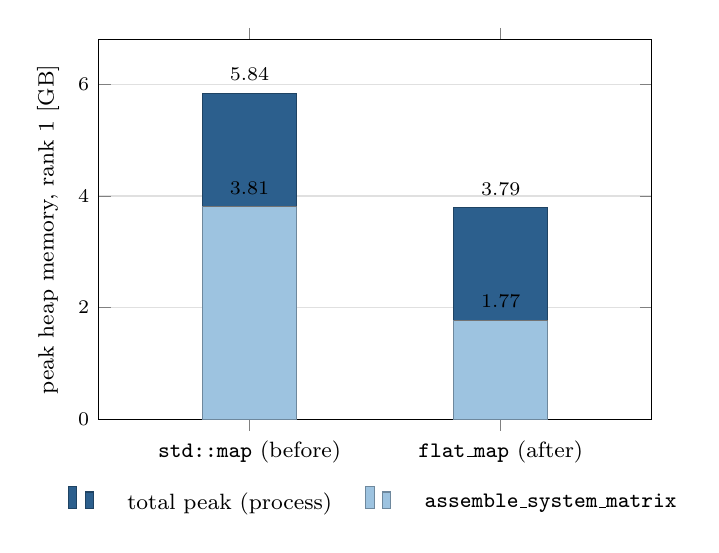
\begin{tikzpicture}
\begin{axis}[
    ybar,
    width=8.6cm, height=6.4cm,
    bar width=34pt,
    xmin=-0.6, xmax=1.6,
    xtick={0,1},
    xticklabels={\texttt{std::map} (before),\texttt{flat\_map} (after)},
    xticklabel style={font=\footnotesize, align=center},
    ymin=0, ymax=6.8,
    ylabel={peak heap memory, rank 1 [GB]},
    ylabel style={font=\footnotesize},
    tick label style={font=\scriptsize},
    ymajorgrids=true,
    major grid style={black!12},
    legend style={
      at={(0.5,-0.16)}, anchor=north, draw=none,
      legend columns=2, font=\footnotesize, column sep=1em,
    },
]
  % Overlay, not stack: assemble_system_matrix is a subset of the total, so the
  % second series is drawn at the same x position (bar shift=0pt) on top of the
  % first, covering its lower portion. The remaining visible strip of memtotal
  % above the seam is "everything in main's peak that is not assembly".
  \addplot+[
    ybar, bar shift=0pt, fill=memtotal, draw=memtotal!70!black, line width=0.4pt,
  ] coordinates {(0,5.84) (1,3.79)};
  \addlegendentry{total peak (process)}
  \addplot+[
    ybar, bar shift=0pt, fill=memassemble, draw=memassemble!70!black, line width=0.4pt,
  ] coordinates {(0,3.81) (1,1.77)};
  \addlegendentry{\texttt{assemble\_system\_matrix}}

  % Value labels: total at the bar top, assemble at the seam between the two
  % colors, with a short cap line marking the seam itself.
  \node[font=\scriptsize, anchor=south, yshift=1pt] at (axis cs:0,5.84) {5.84};
  \node[font=\scriptsize, anchor=south, yshift=1pt] at (axis cs:1,3.79) {3.79};
  \draw[black!55, line width=0.6pt] ([xshift=-17pt]axis cs:0,3.81) -- ([xshift=17pt]axis cs:0,3.81);
  \draw[black!55, line width=0.6pt] ([xshift=-17pt]axis cs:1,1.77) -- ([xshift=17pt]axis cs:1,1.77);
  \node[font=\scriptsize, anchor=south, yshift=1pt] at (axis cs:0,3.81) {3.81};
  \node[font=\scriptsize, anchor=south, yshift=1pt] at (axis cs:1,1.77) {1.77};
\end{axis}
\end{tikzpicture}

\caption[Sparse matrix memory fix]{\textbf{Effect of the \texttt{sparse\_matrix\_template} fix on peak host memory, 6VYB, rank 1.} The process-wide peak heap consumption against the peak attributable to \snakecase{assemble\_system\_matrix} (Section~\ref{sec:evaluation-experimental-setup-comparing-memory-utilization}). Both captures use the LIS solver, measured on the local system (Table~\ref{tab:test-systems}).}
\label{fig:bimpp-memory-fix}
\end{figure}
